\section{Results and Discussion}

\subsection{Static Analysis Tools Effectiveness}
In order to answer this question, we goaled to measure the effective of the studied static analysis tools in terms of precision, false positive rate, running time. We could not measure recall as we do not have all true vulnerabilities in advanced. We utilized the data that produced by our analysis to measure the Running time to measure how long it take one static analysis tool to analyze all studied repositories. In addition, we aimed to Precision and False positive rate as following: 

\begin{equation}
Precision = \frac  {\#TP}{\#TP + \#FP}
\end{equation}


\begin{equation}
False\_positive\_rate = \frac  {\#FP}{\#TP + \#FP}
\end{equation}


Regarding to the running time, as it is shown in Table \ref{SAT}, RATS consumed  264083 millisecond  which is 4.4747 minutes to finish analyzing 40 repositories with multiple checkpoints. Flawfinder took 702497 millisecond which means 11.708 minutes to achieve the same task. Although, Flawfinder generated larger number of warnings compared to RATS. Flawfinder has reported double warnings compared to RATS. Cppcheck consumed  4.597 hours to analyze 40 repositories, however, it did not report any buffer overflow vulnerability.  Table \ref{eff} shows the running time in minutes.



\begin{table}[ht]
\centering
\scriptsize
\caption{The effectiveness studied static analysis tools in terms of precision, false positive rate and runtime.}
\label{eff}
\begin{tabular}{||p{1cm}|p{2cm} p{2cm} p{2cm}||}
\hline
\textbf{Measure} & \textbf{RATS} &	 \textbf{Flawfinder} 	& \textbf{Cppceck} 	\\
\hline\hline
Precision & 0.357&0.537& NA\\
FP\_rate & 0.642 &0.462& NA\\
Runtime & 4.4 & 11.7 &275.8\\
\hline
\end{tabular}
\end{table}

As we can see from Table \ref{eff},  that Flawfinder is slightly more precise than RATS and has less false positive rate.  This could be interesting as Flawfinder produced more number of warnings as well. Hence, further analysis is required to determine where is the findings is true or this could happened due to another reason. Section \ref{ttv} includes more in information in this matter. Though, RATS runtime outperforms other tools. 



\subsection{True Positive Buffer Overflow Vulnerabilities Evolution}
In this section, we were interested in analyzing how did  true positive buffer overflow vulnerabilities evolved over time. In other words,  how long it took repository developers to  detect bugs then removed them from the repository. When we determined a such vulnerability as true positive,  we calculated its age by retrieving the date of the continuous checkpoints that appeared from the first appearance until the last checkpoint that was included. We computed the vulnerability age in month.  Figure~\ref{chart} shows the results obtained. We could see most of the true positives were detected in less than 6 month period of time. However, the chart also shows that there were some vulnerabilities that aged 71 months, about 5 years and 9 months, and then finally removed. In addition, we can see that there are spike at 13 months meaning there were also a number of vulnerabilities stayed undetected for around 2 years. Thus, we conclude that most of true positive are being removed in less than 6 month, however some of true positive vulnerabilities could stay for years without being removed. The result here could be related to the kind of static analysis tools that we studied ( string pattern matching) thus more advanced tools need to examined to reach to more robust conclusion.



\begin{figure} [h!]
\centering
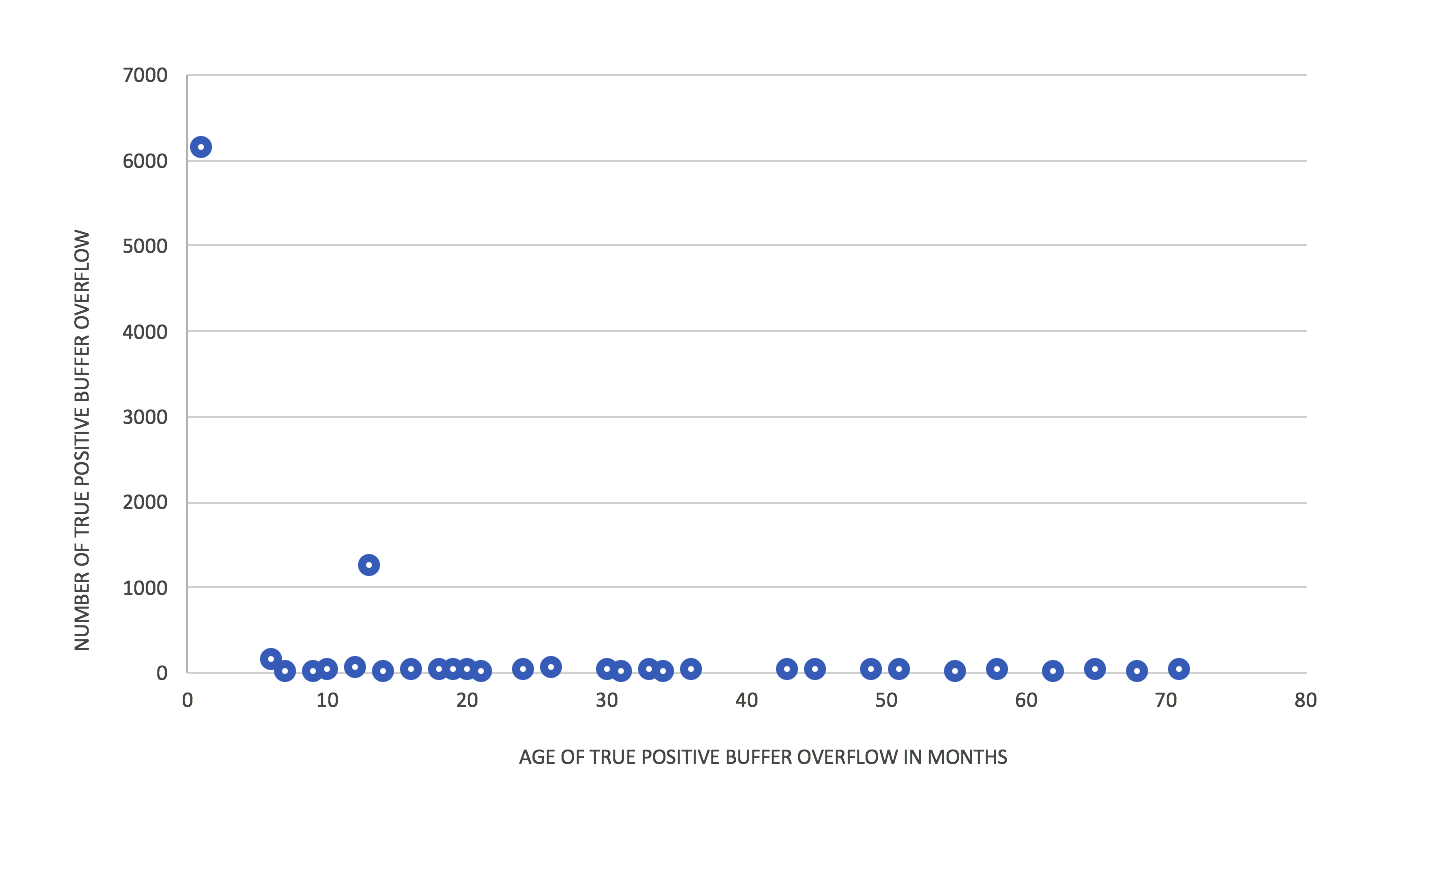
\includegraphics[height=2.5in, width=3.3in]{chart.png}
\caption{True positive buffer overflow vulnerabilities evolution over time}
\label{chart}
\end{figure}




\subsection{True Positive Buffer Overflow Vulnerabilities Patterns}

Finally, we wanted to study which kind of buffer overflow that were determined to be true positive and what pattern that it does hold. By examining all true positive warnings, we found 70 different kinds of warnings that occurred in true positive vulnerabilities. We divide these 70 warnings to three different  categories. The categories are as follow: (1) potentially dangerous function calls, (2) fixed buffer size, and (3) unsensitized input from untrusted source. Table \ref{patterns} shows our findings.




\begin{table}[ht]
\centering
\scriptsize
\caption{The percentages of true positive buffer overflow vulnerabilities patterns.}
\label{patterns}
\begin{tabular}{||p{5cm}|p{2cm} ||}
\hline
\textbf{Pattern} & \textbf{Percentages}  	\\
\hline\hline
Potentially dangerous function calls &  63\% \\
Fixed buffer size & 32\%  \\
Unsensitized input from untrusted source & 5\%\\
\hline
\end{tabular}
\end{table}
